\section{Dedicated Detectors in Future}

Despite a various of researches are done or proposed with superficially comprehensive coverage of LLP at the LHC, there are still cases, including ultra-low-mass particle, ultra-long lifetime particle and , which are barely covered by main experiments at LHC, due to the difficulties in triggering, object reconstruction and event selection. Hence, new proposals for dedicated experiments for LLPs are put forward to fill in these missing pieces. These new experiments are expected to provide good sensitivity to millicharged LLPs, magnetic monopoles and other LLPs hard to trigger or reconstructed.

In general, high mass LLPs with high $p_T$ final states are covered with excellent sensitivity on ATLAS and CMS. Low mass LLPs are more challenging with higher backgrounds and low selection capability of triggers. In the short time regime, as the $c\tau$ comparable with the scale of VErtex LOcator (VELO), the sensitivity extends to lower mass in LHCb. For low-mass LLPs with long-lifetime, few sensitivity can be archived in majar experiments at LHC. LLPs with weak ionization, e.g. millicharged partcle, are barely visible in ATLAS, CMS and LHCb. These signatures can be covered by NA62 operating in beam dump mode, or by dedicated LHC experiments like milliQan, CODEX-b, FASER, or MATHUSLA. Each of dedicated experiments are sensitive to specific type of LLP signature.

\subsection{The milliQan Experiment}

MilliQan is a proposed dedicated experiment conducted at the LHC targeting non-quantized charged particle referred to as \textit{milli-charged particle} (mCP). The milliQan experiment is a segment of a general program to search for hidden sectors and other BSM scenarios. To estimate the potential reach of milliQan from theoretical aspect, an appealing example is built with an extra abelian gauge field added into the SM model. The additional gauge field couples to a massive Dirac fermion ("dark QED") and mixes with hypercharge through the kinetic term:
\begin{equation}
\mathcal{L} = \mathcal{L}_{SM}-\frac{1}{4}A_{\mu\nu}^{\prime}A^{\prime\mu\nu}+i\bar{\psi}(\slashed{\partial}+ie^{\prime}\slashed{A}^{\prime}+ iM_{mCP})\psi-\frac{\kappa}{2}A^{\prime}_{\mu\nu}B^{\mu\nu}
\end{equation}

Eliminating the mixing term by redefining the new gauge boson as $A_{\mu}^{\prime}\rightarrow A_{\mu}^{\prime} + \kappa B_{\mu}$, the coupling of massive charged particle to hypercharge shown as 

\begin{equation}
\mathcal{L} = \mathcal{L}_{SM}-\frac{1}{4}A_{\mu\nu}^{\prime}A^{\prime\mu\nu}+i\bar{\psi}(\slashed{\partial}+ie^{\prime}\slashed{A}^{\prime} - i\kappa e^{\prime}\slashed{B}+ iM_{mCP})\psi
\end{equation}

The new fermion field $\psi$ acts as particle carrying a milli-charge $\kappa e^{\prime}$, the mCP $\psi$ couples to the photon and Z boson with a charge $\kappa e^{\prime}\cos{\theta_W}$ and $-\kappa e^{\prime}\sin{\theta_W}$. The fractional charge in unit of the electric charge is $\epsilon \equiv \kappa e^{\prime} \cos{\theta_W}/e$.

The milliQan apparatus consists of three stacks of 80 cm long plastic scintillator arrays read out by photomultiplier tube (PMT) pointing back to CMS IP, the whole scale of the detector is $3\times1\time1$ m. The experimental signature consists of the photo-electrons (PE) arising from  ionization in the sensitive area produced by mCPs escaping from the LHC detectors. The detector is located in a underground tunnel at LHC P5, which is 33m away from CMS IP, at an angle of 43.1 degrees from the horizontal plane and shielded by 17m length of rock.  

To verify the feasibility  and optimize the design of the detector, around 1$\%$ of the detector is built as a "demonstrator". The demonstrator has been installed and running successfully, and provided valuable data for understanding the background and the performance of the detector. The  charge calibration is essential for milli-charge searches, the calibration is done by calculating the number of PE ($N_{PE}$) for cosmic muons where $N_{PE}$ is extracted by dividing pulse area of cosmic muons by the pulse area of single photon electrons (SPE). Then, the $N_{PE}$ is extrapolated to fractional charge by $Q^2$. The SPEs are taken from late pulses and measured in-situ.  SPE pulse area measurement was also done on the bench as a validation.  The typical value of the measured $N_{PE}$ for $Q= 1e$ is about 5K.  Taking the difference in flight distance of cosmic muons and through-going muons in the scintillator bars(80cm/5cm), the $N_{PE}$ for through-going muon is approximately $5K \times 80/5 =80K$.  This gives $N_{PE}=1$ for $Q \sim 3\times10^{-3}e$, which is consistent with the full Geant4 simulation results. Muons from collisions can help understanding the alignment, trigger and timing calibration.

The dominant background is expected to be the dark current pulses in the PMT. Pulse from background radiation will consist of $\gtrsim 1000$, which can be easily vetoed offline. A triple-incidence within a 15 ns time window along longitudinally contiguous bars in each of the three sections is required to reduce the background from dark-current noise. A full simulation has been performed to evaluate the projected sensitivity to various mCP electric charge and masses, shown in Fig.\ref{fig:mCPsensitivity}

\begin{figure}
    \centering
    \caption{The expected sensitivity of the milliQan experiment
for different LHC luminosity scenarios. The black line shows the
expected $95\%$ C.L. exclusion (solid) and 3$\sigma$ sensitivity (dashed), assuming 300 $fb^{-1}$ of integrated luminosity. In blue is shown the corresponding expectations for 3000 $fb^{-1}$. From Ref.\cite{mCPProposal}}
    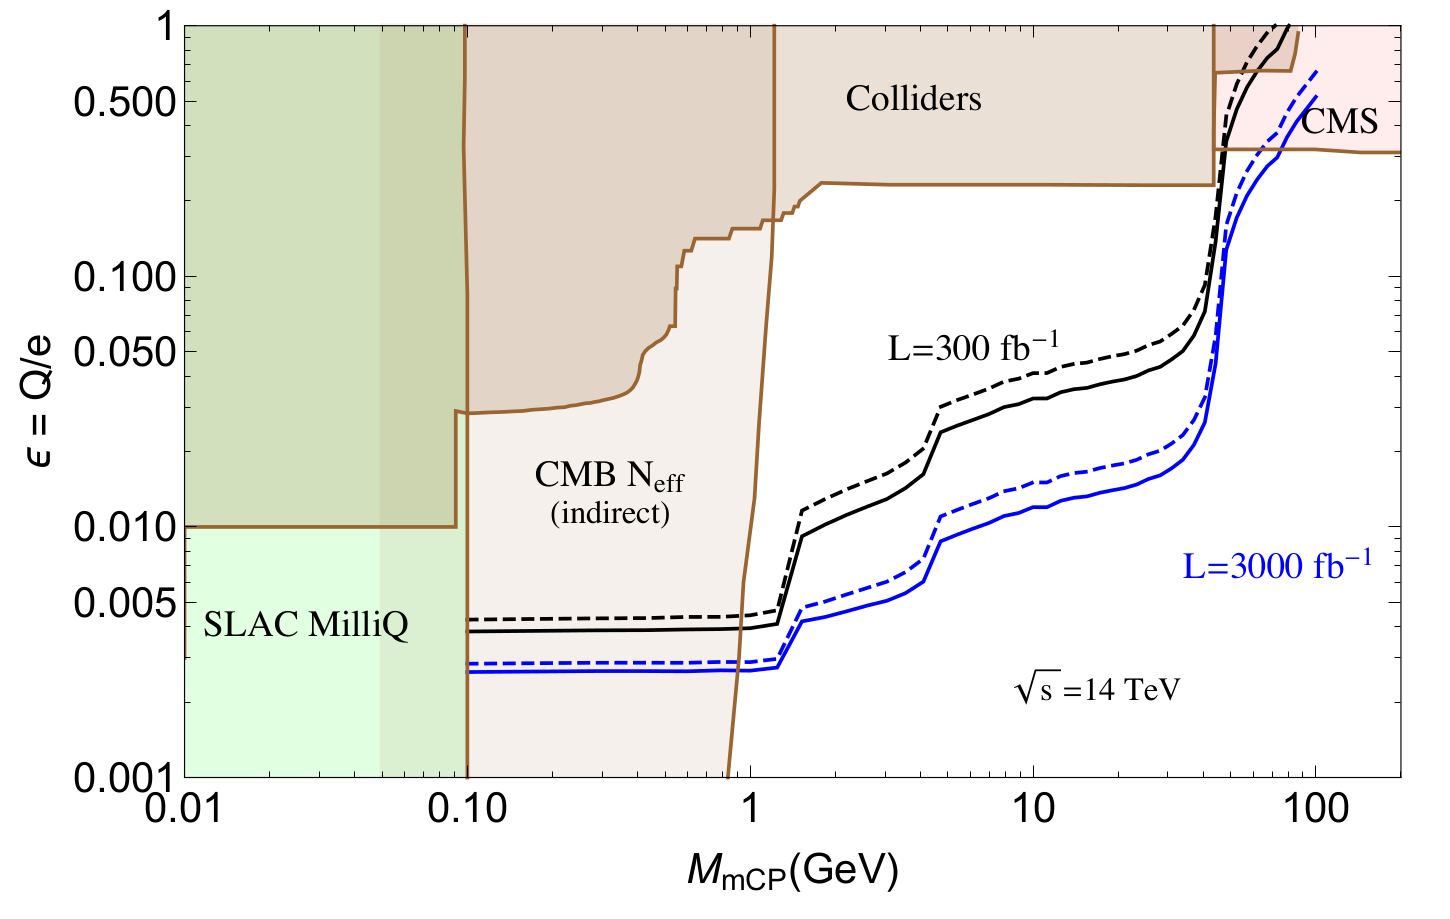
\includegraphics[width=0.5\textwidth]{fig/mCPsensitivity.png}
    \label{fig:mCPsensitivity}
\end{figure}

\subsection{MoEDAL Experiment}

MoEDAL (Monopole and Exotics Detector At the LHC) \cite{MoEDALTDR} is primarily motivated by directly search for the Monopole and other highly ionizing Stable Massive Particles (SMP) at the LHC. A main challenge in highly ionizing particle (HIP) search is the difficulty in $dE/dx$ measurement. The HIP particle can be absorbed before it penetrate the whole detector, or the $dE/dx$ measurement will be problematic due to saturation of the electronics in the tracker system. The MoEDAL experiment is proposed to complement the search capabilities of the general purpose LHC detectors, allowing searches for electrically and magnetically charged SMPs with $Z/\beta$- actual or effective - potentially as low as 5, where Z is the electric charge.

The MoEDAL detector is comprised of an array of plastic Nuclear Track Detectors (NTDs), located around the intersection at LHC Point8 (IP8) in the LHCb VELO cavern. The schematic view of the MoEDAL experiment is shown in Fig.\ref{fig:MoEDALgeometry}. The array consists of NTD stacks, nine layers deep, in Aluminium housings attached to the walls and ceiling of the VELO cavern. The maximum possible surface area available for detectors is around 25 $m^2$. The signatures of HIP are analyzed with invisible damage zone, which revealed as a cone-shaped etchpit, along the trajectory.

\begin{figure}
    \centering
    \caption{A 3D schematic view of the MoEDAL detector (in the yellow circle) around the LHCb VELO region at Point 8 of the LHC}
    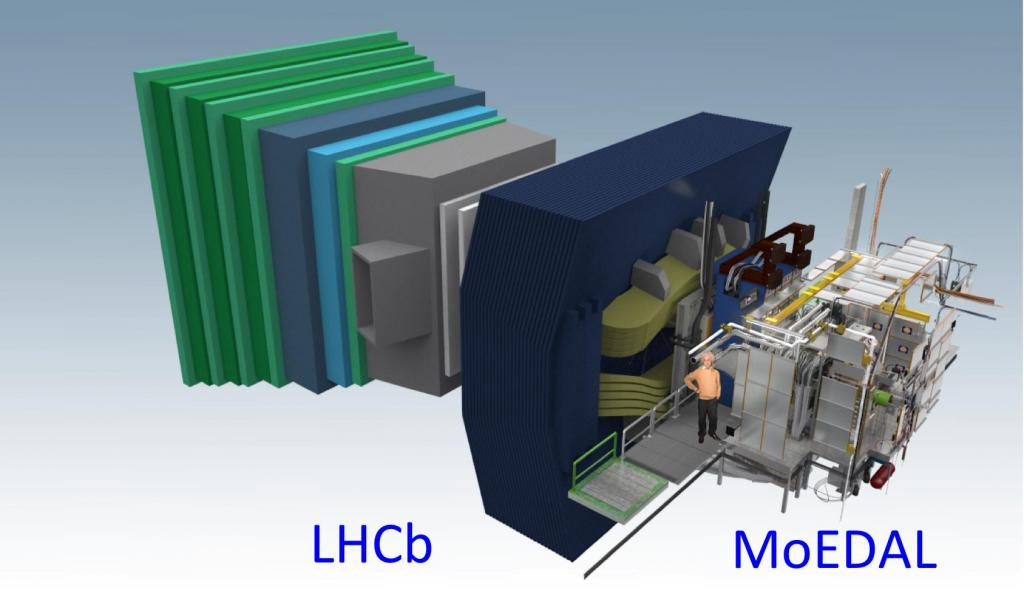
\includegraphics[width=0.5\textwidth]{fig/MoEDAL.png}
    \label{fig:MoEDALgeometry}
\end{figure}

\subsection{The MATHUSLA Experiment}
The goal of the MATHUSLA (MAssive Timing Hodoscope for Ultra-Stable neutraL pArticles) detector is the search for LLPs with lifetimes much larger than the size of the LHC main detectors,$c\tau \ll 100$ m. With the limit on the scale of the detector, only a small fraction of such LLPs can be found decaying in the sensitive volume of the detector. MATHUSLA is proposed to be a large, relatively simple surface detector that can robustly reconstruct DVs with good timing resolution. The simplified illustration of MATHUSLA is shown in Fig.\ref{fig:MATHUSLA}.

\begin{figure}
    \centering
    \caption{Simplified MATHUSLA detector layout showing the position of the 200 m $times$ 200 m $times$ 20 m LLP decay volume.}
    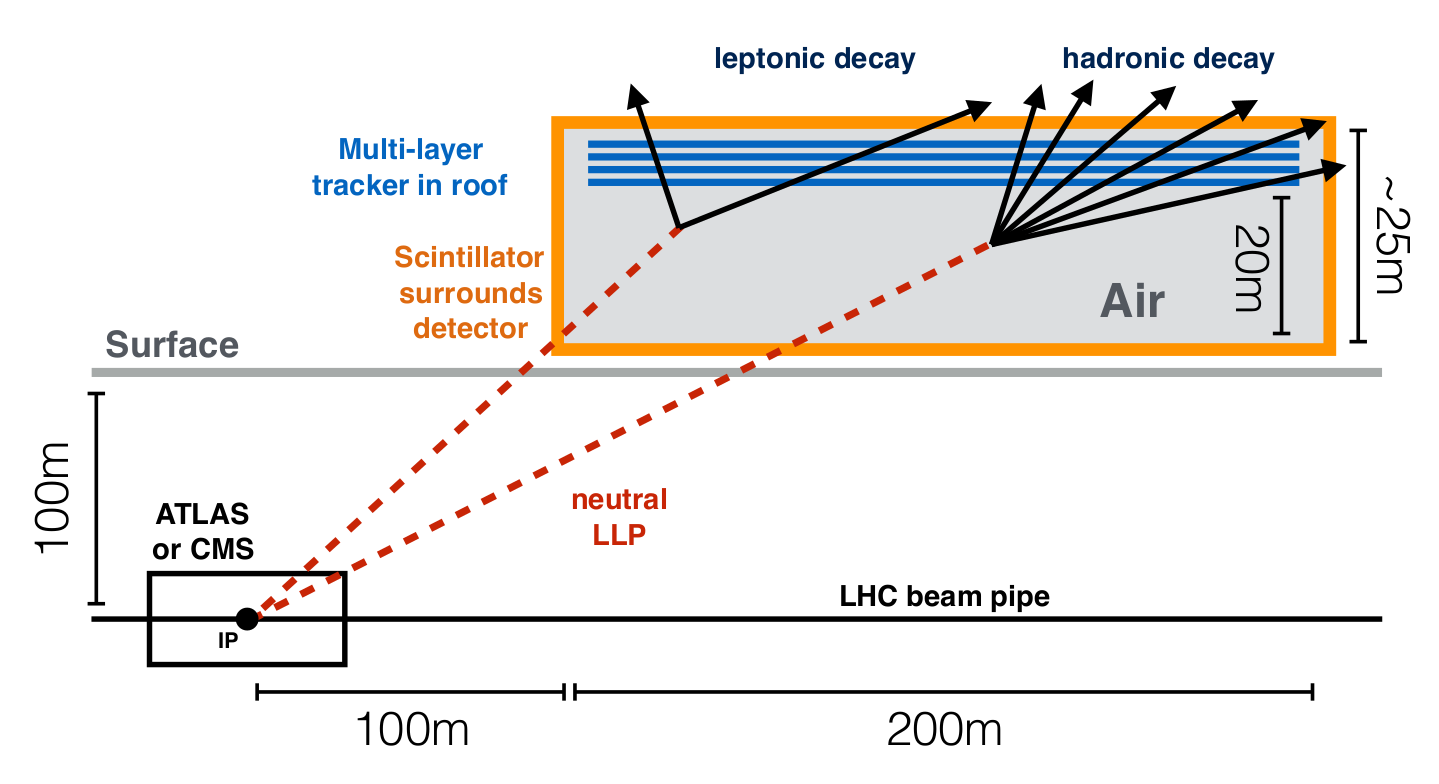
\includegraphics[width=0.5\textwidth]{fig/MATHUSLA.png}
    \label{fig:MATHUSLA}
\end{figure}

It is a large-scale detector composited with a tracker array situated above an air-filled decay volume that is 20 m tall and 200 m $\times$ 200 m in area. The tracker layers provide robust tracking with $\sim$ns timing and $\sim$cm spatial resolution. The trackers are implemented with Resistive Plate Chambers (RPCs) technology to make the balance between functionality and economy. MATHULSLA can improve the sensitivity to these LLP production
cross sections by a factor of $\sim 10^3$ for LLPs with masses $\lesssim 100$ GeV that decay hadronically and without associated production of other highly visible signals. 

In summary, the MATHUSLA detector is proposed as a dedicated LLP surface detector with large sensitive volume and potentially improve the sensitivity by several orders of magnitude for many LLP scenarios. A small-scale demonstrator are installed and taking data at LHC.
